\subsection{Evaluating Adverse Externalities}
Evaluating adverse externalities helps regulators determine whether or not an insolvent bank should be liquidated through the Federal Bankruptcy Code.  If adverse externalities could endanger the public good, then the insolvent financial firm undergoes either a special liquidation process or is made solvent thought the direct injection of liquidity supported by the government.  Deciding whether or not a financial firm should be ``saved'' through direct liquidity injection supported by the government is a matter of assessing how large the adverse externalities; a firm is 'saved' if it is Too Big To Fail (TBTF).  

If the financial firm could fail conventionally through the FBC without giving rise to some viscous downward spiral of asset value, then the insolvent firm is conventionally liquidated.  TBTF has been applied particularly in finance, because losses suffered by some large counterparties of an insolvent large firm, including other financial firms, may have disproportionately large adverse externalities on the economy served by the bank.\cite{Kaufman}

A particular set of adverse externalities is portrayed below by William Dudley, President of the Federal Reserve Bank of New York (FRBNY):

\indent {"The root cause of ``Too Big To Fail'' is the fact that in our financial system as it exists \\ \indent today, the failure of large complex financial firms generate large, undesirable externali- \\ \indent ties. These include disruption of the stability of the financial system and its ability to  \\ \indent provide credit and other essential financial services to households and businesses. When  \\ \indent this happens, not only is the financial sector disrupted, but its troubles cascade over  \\ \indent into the real economy.\cite{Dudley}}

\noindent Proponents of government intervention, such as FRBNY President William Dudley, argue that the wealth of average americans and the strength of the economy come above all else in these TBTF situations.  The opposition to government intervention, in these TBTF situations, argue that when government gets involved there is an erosion of market discipline and a disruption in free market asset valuation.

\subsection{Lender of Last Resort}
%%%%Next section%%%%%%   Why the government must step in, for all of time
In the United States, the regulators are allowed to deviate from the least cost resolution principle in the case of failure of an ``essential'' financial firm.\cite{Rime}  Essential firms can be those that follow up bankruptcy liquidation with an economy wide viscous downward spiral in asset value.  Essential firms can also be those in the ``public interest,'' such as those firms supplying credit and debt servicing.  It is very difficult to weigh the importance of these ``public interest'' financial firms.\cite{Kaufman}  However, it is clear that the regulators and United States government only act to protect the wealth of the average american and the debt services that emanate from the financial firm business.  The government and its regulators have hinted at TBTF by mentioning exceptions to the rules for ``essential'' and ``public interest'' financial firms.


%4)capitalism and how third party saviors will always be looking to make money and not protect the liquidation downward spiral of assets; 
%5)sequence of events in liquidation and how this is harmful; 
%
%%\subsection{Historical TBTF}  %Historical Precedence of Bailouts/TBTF  - Andrew and Grant
%6) Historical precedence of being on the edge, or govt. thinks we are on the edge, of a downward asset spiral.
%
%
%The adverse economic impact of the failure of such ?shadow? banks also has increasingly come to be viewed as similar to that generated by the failure of large commercial banks13. That is, some large nonbank financial companies are increasingly perceived to be as ?special? as large commercial banks in terms of the characteristics discussed earlier. Indeed, until the enactment of DFA, the damage from their failure may have even been greater since the failures were generally resolved under the Federal Bankruptcy Code, which was viewed by many as economically less efficient, more costly, and more disorderly than the resolution process for large banks under the FDIA (Board of Governors, 2011)14
%
%
%The demeanor change - increasing seriousness of the govt action(continental and FDICIA), 
%allow the depositors to take a loss but only if it feels that the negative externalities of the failure will not endanger the wealth of many people; 
%

%why does government step in as the last option third party/resort


\subsection{Examples Abroad} 
In the context of system-wide crises, the governments of Japan, Sweden, Finland and Norway have granted blanket state guarantees to all financial firms, regardless of their size.\cite{Rime}  These nations understand the intimate connection between a viscous downward spiral in asset value, and the corresponding downward spiral in personal wealth.  With smaller nations, giving blanket coverage to all financial firms in the economy bolsters the supply of credit and protects the reputation of the smaller economies.\cite{Rime}

\begin{figure}[H]
\centering
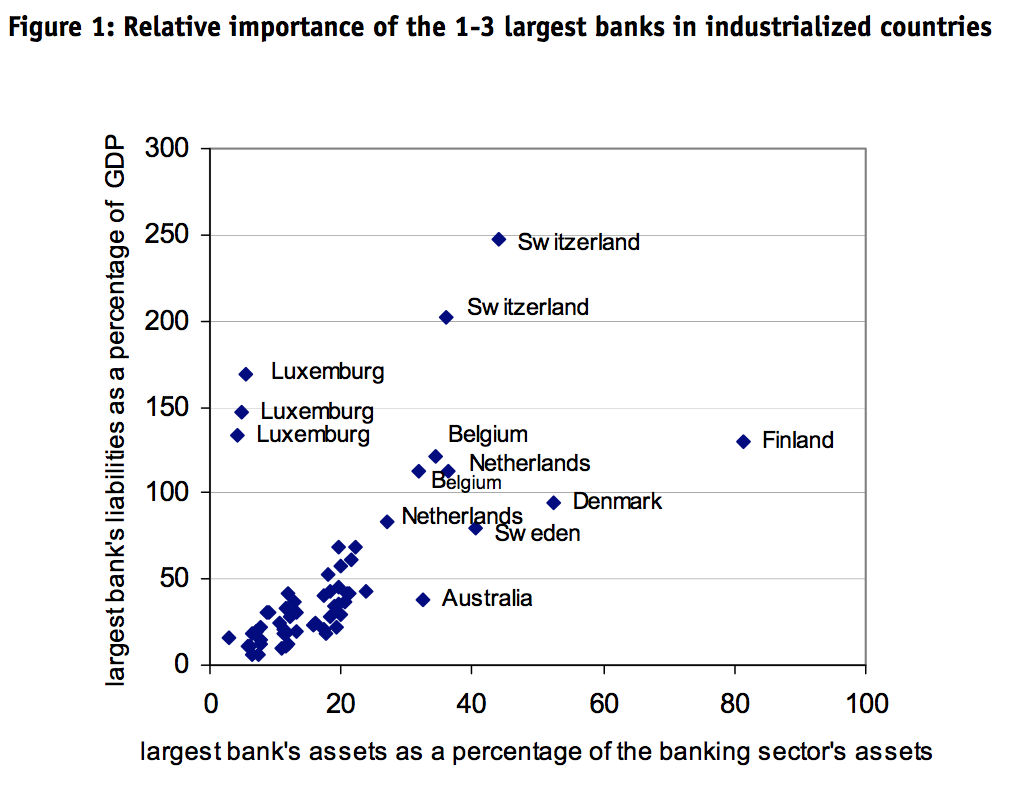
\includegraphics[scale=.70]{figure/RimeForeigners.png}\\[-0.7cm]
\caption{Leverage in Foreign Financial Firms\label{fig:abroad}}
\end{figure}

In figure \ref{fig:abroad}, the asset value of the top three financial firms in a variety of nations is close to the entire economy's gross domestic product.  A downward spiral in the asset value at these financial firms could create losses the size of the national gross domestic product, and cripple their national economies.  In order to protect the financial firms from having to fire sell their assets in a liquidity squeeze the government explicitly guarantees these illiquid assets, in turn protecting the wealth of their citizens and the wealth of the global economy.  As an extrapolation from the illiquid asset protection guaranteed under the FDIC in the United States, these foreign nations have begun explicit backing enormously leveraged financial firms.
